\documentclass[]{rAMF2e}
%\usepackage[square]{natbib}
%\usepackage{authblk}
\usepackage{listings}
\usepackage[center]{caption}
\usepackage{hyperref}


\begin{document}
\doi{}
\issn{}  \issnp{}
\jvol{00} \jnum{00} \jyear{2013} %\jmonth{January--March}
\def\jobtag{}
\publisher{Unpublished}
\jname{}

\markboth{Fabien {Le Floc'h}}{Draft}

\title{Fast and Robust SABR Calibration through Simple Expansions}
\author{Fabien {Le Floc'h}$^\star$\thanks{{\em{Correspondence Address}}: Calypso Technology, 106 rue de La Bo\'{e}tie, 75008 Paris. Email: \texttt{fabien\_lefloch@calypso.com}}
\affil{$^\star$Calypso Technology, 106 rue de La Bo\'{e}tie, 75008 Paris}}
%
\date{\today}
\received{v1.0 released June 2014}

\maketitle
\newcommand{\sgn}{\mathop{\mathrm{sgn}}}
\begin{abstract}
The SABR stochastic volatility model is a very popular interpolator of implied volatilities, with a given dynamic. This paper presents a simple and very fast method to calibrate the SABR model to given market volatilities, that is to imply the SABR parameters from a given market smile.
\begin{keywords}stochastic volatility, SABR, calibration, implied volatility, finance\end{keywords}
\end{abstract}

\section{Introduction}
The SABR stochastic volatility model \citep{hagan2002managing} enjoys a high popularity as interpolator of implied volatilities, because, in practice, it fits rather well market implied volatility smiles for interest rate derivatives, fx derivatives and equity derivatives with a few parameters $\alpha, \rho, \nu$, and the dynamic of it can be easily controlled through its $\beta$ parameter, usually defined from historical series analysis for the relevant market.

There are however known shortcomings: it is not arbitrage free as the probability density can become negative for low strikes and long maturities. Many authors have proposed various improvements to the original formula \citep{obloj2008fine, johnson2009arbitrage, paulot2009asymptotic, benaim2008arbitrage}. More recently the focus has been on finite difference techniques to guarantee the arbitrage-free property \citep{hagan2013arbitrage,lefloch2014fdmsabr} in a shifted SABR framework, to allow for negative rates. 

In practice, the adjustments to the original formula don't matter much in order to find a good initial guess for the calibration procedure. Once a good initial guess is found, a fast local minimizer like Levenberg-Marquardt can be used to calibrate the specific SABR implementation. 

A first calibration method was described in \citep{west2005calibration}, fitting $\alpha$ exactly to the at-the-money implied volatility, and reducing the problem to a two-dimensional minimization in $(\rho,\nu)$. The Nelder-Mead method is proposed as minimizer. It however still requires some initial guess, and can sometimes be unstable, especially with constraints \citep{lefloch2014nelder}. A numerical method to find an initial guess that fits exactly the at-the-money volatility and the at-the-money skew is proposed in \citep{gauthier2009fitting}. It requires however to solve numerically a two-dimensional non linear system of equations.

In contrast, the method proposed here consists in solving analytically a simple system of equations to fit the at-the-money volatility, skew, and curvature. A similar approach was applied to the Heston model in \citep{forde2012small} with the difference that, in their case, the Heston parameters describe a full volatility surface and the initial guess procedure relies on two expiries plus the short time at-the-money volatility to solve the 5 Heston parameters exactly. In the SABR case, there is just one expiry to consider and 3 parameters to fit. We will first present our method for the lognormal formula as well as for the normal formula, and then show its accuracy in calibrating real world smiles on the arbitrage-free model from \citet{hagan2013arbitrage} compared to a global optimization via differential evolution.


\section{SABR normal and lognormal formulas}
%The advantage to rely on the original formula is speed, as it is usually much faster to evaluate than the alternatives. For lognormal (Black) volatilities, we prefer the formula from Obloj \citep{obloj2008fine} as it is seen as more consistent. For normal (bpvol) volatilities, we rely on the Hagan formula in \citep{hagan2002managing} as it has no such inconsistency.

\subsection{The SABR model}
In the shifted SABR model, the asset forward follows the following stochastic equation:
\begin{align}
dF &= V (F+b)^\beta dW_1\\
dV &= \nu V dW_2
\end{align}
with $W_1, W_2$ Brownian motions correlated with correlation $\rho$,
and $F(0) = f$, $V(0) = \alpha$.
$\nu$ represents the volatility of volatility, $b$ is a displacement allowing for negative rates ($b=0$ for the classic SABR model).

\subsection{Normal formula}
Taking into account the remarks from \citet{obloj2008fine} for the case of the lognormal formula to ensure consistency when $\beta \to 1$, the expansion of the normal volatility adapted from \citet{hagan2002managing} for the shifted SABR model is:

for $f \neq K$ and $\beta \in [0,1]$
\begin{align}
\sigma_N(K) &= \frac{f-K}{x(K)}\left[1+\left(g(K)+\frac{1}{4}\rho\nu\alpha\beta(f+b)^{\frac{\beta-1}{2}}(K+b)^{\frac{\beta-1}{2}}+\frac{1}{24}(2-3\rho^2)\nu^2\right)T\right]
\end{align}
with 
\begin{align*}
g(K) &= \frac{1}{24} (\beta^2-2\beta) (f+b)^{\beta-1} (K+b)^{\beta-1} \alpha^2\\
\zeta(K) &= \frac{\nu}{\alpha (1-\beta)} \left( (f+b)^{1-\beta} - (K+b)^{1-\beta} \right)\\
x(K) &= \frac{1}{\nu}\log\left(\frac{\sqrt{1-2\rho\zeta(K)+\zeta^2(K)}-\rho+\zeta(K)}{1-\rho} \right)
\end{align*}

When $f=K$, 
\begin{align}
\sigma_N(f) &= \alpha (f+b)^\beta \left[1+\left(g(f)+\frac{1}{4}\rho\nu\alpha\beta(f+b)^{\beta-1}+\frac{1}{24}(2-3\rho^2)\nu^2\right)T\right]
\end{align}

When $\beta = 1$,
\begin{align*}
g(K) = -\frac{1}{24}\alpha^2 &\texttt{ , } \zeta(K) = \frac{\nu}{\alpha} \log\left(\frac{f+b}{K+b}\right)
\end{align*}

When $\beta = 0$,
\begin{align*}
g(K) = 0 &\texttt{ , }\zeta(K) = \frac{\nu}{\alpha} \left(f-K\right)
\end{align*}
%recap of SABR Hagan 2002 formula and obloj
\subsection{Lognormal formula}
The lognormal formula is very similar to the normal formula, $f-K$ becomes $\log(\frac{f}{K})$ and $g$ includes a small adjustment:

for $f \neq K$ and $\beta \in [0,1]$,
\begin{align}
\sigma_B(K) &= \frac{1}{x(K)}\log(\frac{f+b}{K+b})\left[1+\left(g(K)+\frac{1}{4}\rho\nu\alpha\beta(f+b)^{\frac{\beta-1}{2}}(K+b)^{\frac{\beta-1}{2}}+\frac{1}{24}(2-3\rho^2)\nu^2\right)T\right]
\end{align}
with 
\begin{align*}
g(K) &= \frac{1}{24} (\beta-1)^2 (f+b)^{\beta-1} (K+b)^{\beta-1} \alpha^2\\
\zeta(K) &= \frac{\nu}{\alpha (1-\beta)} \left( (f+b)^{1-\beta} - (K+b)^{1-\beta} \right)\\
x(K) &= \frac{1}{\nu}\log\left(\frac{\sqrt{1-2\rho\zeta(K)+\zeta^2(K)}-\rho+\zeta(K)}{1-\rho} \right)
\end{align*}

When $f=K$, 
\begin{align}
\sigma_B(f) &= \alpha (f+b)^{\beta-1} \left[1+\left(g(f)+\frac{1}{4}\rho\nu\alpha\beta(f+b)^{\beta-1}+\frac{1}{24}(2-3\rho^2)\nu^2\right)T\right]
\end{align}

When $\beta = 1$,
\begin{align*}
g(K) = 0 &\texttt{ , } \zeta(K) = \frac{\nu}{\alpha} \log\left(\frac{f+b}{K+b}\right)
\end{align*}

When $\beta = 0$,
\begin{align*}
g(K) = \frac{1}{24(f+b)(K+b)}\alpha^2 &\texttt{ , }\zeta(K) = \frac{\nu}{\alpha} \left(f-K\right)
\end{align*}
It is important not to forget that Hagan derived the lognormal formula as an approximation of the normal formula \citep{hagan2002managing}: it won't be accurate or realistic at all in cases where the implied volatility is very high (see Table \ref{tbl:lognormal_high_alpha}). This is not so realistic for market implied volatilities, but it can have an influence in the global minimization procedure, as global minimizers like differential evolution will try out extreme values.

Of course, in order to obtain a lognormal volatility, it is also possible to solve with high accuracy for the Black implied volatility of a given normal volatility: we can firstly compute corresponding Bachelier option price with a fast evaluation method (see appendix) and secondly use a robust and accurate Black implied volatility solver \citep{jackel2013let, li2011adaptive}.

\begin{table}[h]
\begin{center}
\caption{\label{tbl:lognormal_high_alpha}Black volatility obtained from the direct lognormal approximation compared the one solved from the normal approximation using $\alpha=3.24,\beta=1.0,\rho=-0.998, \nu=1.69, f=2014, K=f, T=0.48$.}
\begin{tabular}{|c|c|c|}
\hline
Formula & Black volatility & Option price \\ 
\hline
Lognormal & 0.9325 & 510.19 \\
Normal & 0.2526 & 140.41 \\
\hline
\end{tabular}
\end{center}
\end{table}
%bachelier price can be infinite when bachelier vol high, while blackscholes is 0
%solving can break down in those cases.
For performance reasons, we prefer to rely on the normal formula if the calibration is for bpvols and the lognormal formula if the calibration is for Black volatilities.

\subsection{Latest Hagan normal formula}
%mention of latest Hagan formula 2014

\section{Explicit initial guess}
\subsection{Lognormal volatility}
The idea is to find $\alpha, \rho, \nu$ that matches the at-the-money implied volatility $\sigma_0$, skew $\sigma_0'$ and curvature $\sigma_0''$. Hagan formula would lead to a system of trivariate polynomials of degrees 3 and 4, which would then require a numerical method. Instead, we rely on simpler lower order lognormal volatility expansions obtained with the formula from \citep{lorig2014implied}. Applied to the shifted SABR model, their second order expansion of the implied volatility $v$ is $v = v_0 + v_1 + v_2$ where 
%lorig formula for order 2 %
\begin{align*}
v_0 &= \alpha (f+b)^{\beta-1}\\
v_1 &= \frac{1}{2}(\beta-1) z v_0 + \frac{1}{2}z\rho\nu+ \frac{1}{4}T\nu v_0(\rho v_0 - \nu)\\
v_2 &= \frac{1}{96}(\beta-1)^2 v_0 \left(8z^2+T v_0 (4-T v_0^2)\right)\\
&- \frac{1}{48}T(\beta-1)\nu v_0 \left(6z\nu+2(6-5z)\rho v_0 + T\rho v_0^3\right)\\
&+ \frac{1}{96}T\nu^2 v_0 \left(32 + 5T\nu^2 - 12 \rho^2 + 2T v_0((6\rho^2-2)v_0-7\nu\rho) \right)\\
&- \frac{1}{24}T\nu^2\rho (\nu-3\rho v_0) z+\frac{\nu^2(2-3\rho^2)}{12}z^2
\end{align*}
 We use the order-0 expansion for the at-the-money implied volatility, the order-1 expansion for the at-the-money skew, and the order-2 for the at-the-money curvature and ignore terms quadratic in time to expiry $T^2$. Note that the derivatives are expressed in log-moneyness towards the variable $z=\log(\frac{K+b}{f+b})$ where $K$ is the strike and $f$ is the forward. We have then:
\begin{align}
\alpha &= \sigma_0 (f+b)^{1-\beta}\\
\sigma_0' &= \frac{1}{2}\left(\rho \nu - (1-\beta)\sigma_0\right)\\
\sigma_0'' &= \frac{1}{3\sigma_0}\nu^2+\frac{1}{6\sigma_0}\left((1-\beta)^2\sigma_0^2 + 3\rho^2\nu^2\right)
\end{align} 

This system can be exactly solved to give a first guess $\alpha_0, \rho_0,\nu_0$:
\begin{align}
\alpha_0 &=  \sigma_0 (f+b)^{1-\beta}\\
\nu_0^2 &= 3\sigma_0\sigma_0''-\frac{1}{2}(1-\beta)^2\sigma_0^2+\frac{3}{2}\left(2\sigma_0'+(1-\beta)\sigma_0\right)^2 \\
\rho_0 &= \frac{1}{\nu_0}\left(2\sigma_0'+(1-\beta)\sigma_0\right)          
\end{align}
We make sure to constrain $\nu_0$ to be strictly positive (for example by flooring it to $10^{-4}$) , and $\rho_0$ to be in [-1,1]. We then refine this first guess by solving exactly for the at-the-money volatility with the given $\rho_0$ and $\nu_0$. $\alpha_1$ is the root of the following third order polynomial:
\begin{align}
\frac{(1-\beta)^2 T}{24 f^{2-2\beta}}\alpha^3+ \frac{\rho\beta\nu T}{4f^{1-\beta}}\alpha^2 + \left(1+\frac{2-3\rho^2}{24}\nu^2 T\right)\alpha - \sigma_0 f^{1-\beta} &= 0
\end{align}
This is the same polynomial used by \citet{west2005calibration} to reduce the dimension of the calibration problem. $\alpha_1$ is picked as the smallest positive root. In theory, choosing the $\alpha_1$ closest to the previously calibrated $\alpha$ (either from the previous expiry, or from a previous day) could be better. In practice, it turns out to always be the smallest positive root. We then compute $\nu_1, \rho_1$ based on this new $\alpha_1$.
\begin{align}
\sigma_1 &=  \alpha_1 (f+b)^{\beta-1}\\
\nu_1^2 &= 3\sigma_1\sigma_0''-\frac{1}{2}(1-\beta)^2\sigma_1^2+\frac{3}{2}\left(2\sigma_0'+(1-\beta)\sigma_1\right)^2 \\
\rho_1 &= \frac{1}{\nu_1}\left(2\sigma_0'+(1-\beta)\sigma_1\right)          
\end{align}

\subparagraph{How to find the at-the-money volatility, slope and curvature?} The simplest is to fit a parabola to the three closest points around the forward with coordinates $(z_{-1}, \hat{\sigma}_{-1}), (z_0,\hat{\sigma}_0), (z_{1},\hat{\sigma}_1)$. This is equivalent to a 3 points finite difference on a non uniform grid. We have then:
\begin{align}
\sigma_0 &= z_0 z_1 w_{-1} \hat{\sigma}_{-1} + z_{-1} z_1 w_{0} \hat{\sigma}_{0} +  z_{-1} z_0w_{1} \hat{\sigma}_{1}\\
\sigma_0' &= -(z_0 + z_1) w_{-1} \hat{\sigma}_{-1} - (z_{-1}+ z_1) w_{0} \hat{\sigma}_{0} -  (z_{-1}+ z_0)w_{1} \hat{\sigma}_{1}\\
\sigma_0'' &= 2 w_{-1} \hat{\sigma}_{-1} +2 w_{0} \hat{\sigma}_{0} + 2w_{1} \hat{\sigma}_{1}
\end{align}
with 
\begin{align}
w_{-1} &= \frac{1}{(z_{-1}-z_{0})(z_{-1}-z_{1})}\\
w_{0} &= \frac{1}{(z_{0}-z_{-1})(z_{0}-z_{1})}\\
w_{1} &= \frac{1}{(z_{1}-z_{-1})(z_{1}-z_{0})}
\end{align}
In our experience, using higher order approximations like a 5 points finite difference (equivalent to a quartic on 5 points), or a cubic spline does not lead to any visible improvement in accuracy on our problem.
 
When the input data is noisy, one could resort to a best fit parabola around the five closest points from the forward, which can be reduced to solving simple linear system. When the volatility at the forward is already present in the input data, we make sure the parabola passes exactly through it.

Another approach is to repeat the initial guess procedure with a parabola on different sets of three points further away from the forward and select the guess corresponding to the best overall fit.

In our numerical tests we will select the guess that gives the minimum mean square error in volatilities between the two guesses stemming from the 3-points parabola and the 5-points parabola.

\subsection{Normal volatility}
When the input volatilities are normal (bpvol), we just convert them to equivalent lognormal volatilities and apply the same method as in the previous section to find the initial guess.


A normal volatility $\sigma_N$ can be converted almost exactly to a lognormal volatility $\sigma_B$ by first pricing an out of the money option with the Bachelier formula, and inverting the price to find the lognormal volatility with an accurate solver \citep{jackel2013let}. 
In our case, because the initial guess method depends mostly on volatilities closest to the money, we can also rely on another simple expansion based on the work of \citep{lorig2014implied}:
\begin{align}
\sigma_B &= v_0 - \frac{1}{2}v_0 z + \frac{1}{96}v_0(8z^2+T v_0^2 (4-T v_0^2)) \\
         &+ \frac{1}{192}T z v_0^3 (-12+5T v_0^2)
\end{align}
with $v_0 = \frac{\sigma_N}{f}$ and $z=\log(\frac{K}{f})$, where the last term is of order-3.
\section{Almost exact inversion of SABR smiles}
We use the SABR parameters found by calibration on the S\&P500 options in December 2008 as starting point (Table \ref{tbl:smart_initialguess_sabr_input}). From those we regenerate a discrete set of implied volatilities for 12 strikes and 11 expiries using the lognormal SABR formula with $\beta = 1$. And finally we apply our initial guess procedure to each expiry.
\begin{table}[h]
\begin{center}
\caption{\label{tbl:smart_initialguess_sabr_input}Reference SABR parameters}
\begin{tabular}{|c|c|c|c|}
\hline
Expiry & $\alpha$ & $\rho$ & $\nu$ \\ 
\hline
0.058&	0.271&	-0.345&	1.010 \\
0.153&	0.256&	-0.321&	0.933\\
0.230&	0.256&	-0.346&	0.820\\
0.479&	0.255&	-0.370&	0.629\\
0.729&	0.257&	-0.403&	0.528\\
1.227&	0.260&	-0.429&	0.448\\
1.726&	0.261&	-0.440&	0.392\\
2.244&	0.262&	-0.445&	0.355\\
2.742&	0.262&	-0.445&	0.329\\
3.241&	0.262&	-0.447&	0.310\\
4.239&	0.263&	-0.452&	0.284\\
\hline
\end{tabular}
\end{center}
\end{table}

The root mean square error in implied volatilities of the fit is always lower than $3\cdot 10^{-4}$. $\rho, \nu$ are recovered with an accuracy higher than $5\cdot 10^{-3}$ and $\alpha$ is recovered with and accuracy higher than $10^{-4}$, independently of the expiry (see Figure \ref{fig:smart_initialguess_sabr_input}). 
\begin{figure}[htbp]
  \caption{\label{fig:smart_initialguess_sabr_input}Error between the initial guess and the original SABR parameters}
\begin{center}
 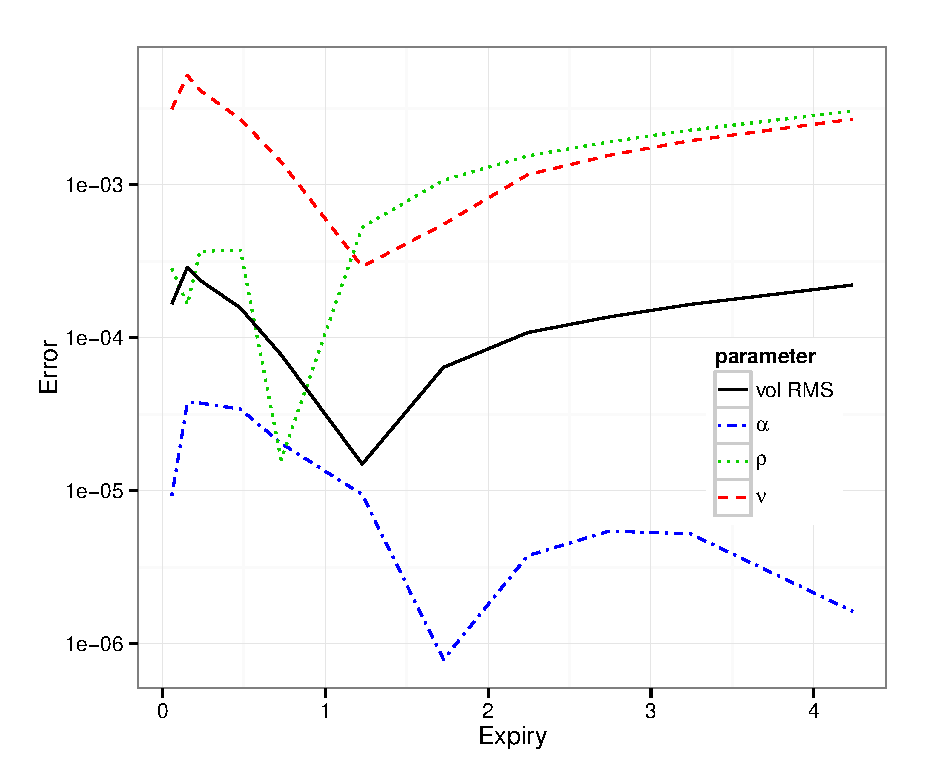
\includegraphics[width=10cm]{smart_initialguess_sabr_input.eps}
\end{center}
\end{figure}

\section{Real world smiles}
\subsection{Calibration on the analytic formula}
\subsubsection{Equity option smiles}
To calibrate SABR to equity implied volatility surfaces, we minimize the root mean square error in implied volatilities with the Levenberg-Marquardt method \citep{}, using as initial guess, either our explicit method, or alternatively a guess found by running the differential evolution algorithm \citep{} with a population size 20 on 1000 generations. The resulting mean square error is displayed in Figure \ref{fig:explicit_de_equity_error}.

\begin{figure}[htbp]
  \caption{\label{fig:explicit_de_equity_error}Root mean square error of calibration on various equity surfaces}
\begin{center}
 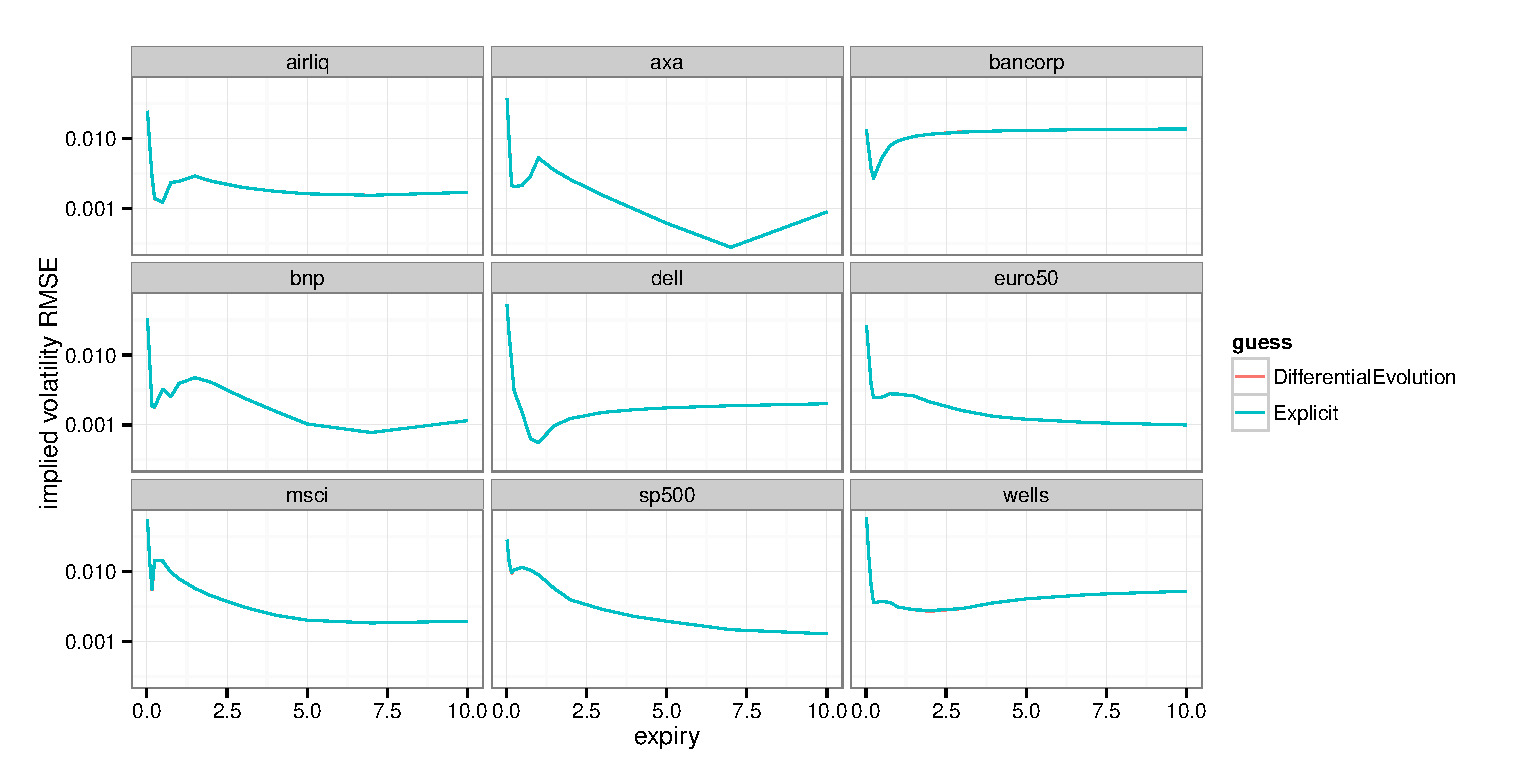
\includegraphics[width=12cm]{explicit_de_equity_error.eps}
\end{center}
\end{figure}

The explicit guess leads a mean square error in implied volatilities nearly indistinguishable from the differential evolution guess. It is interesting however to look at the calibrated parameters values: the calibrated $\alpha$ shows some strong variations with the guess found by differential evolution, while it is relatively smooth with our explicit initial guess (Figure  \ref{fig:explicit_de_equity_alpha}). $\rho$ and $\nu$ behave similarly. We will take a closer look at why this happens in the next section.
\begin{figure}[htbp]
  \caption{\label{fig:explicit_de_equity_alpha}Calibrated $\alpha$ on various equity surfaces}
\begin{center}
 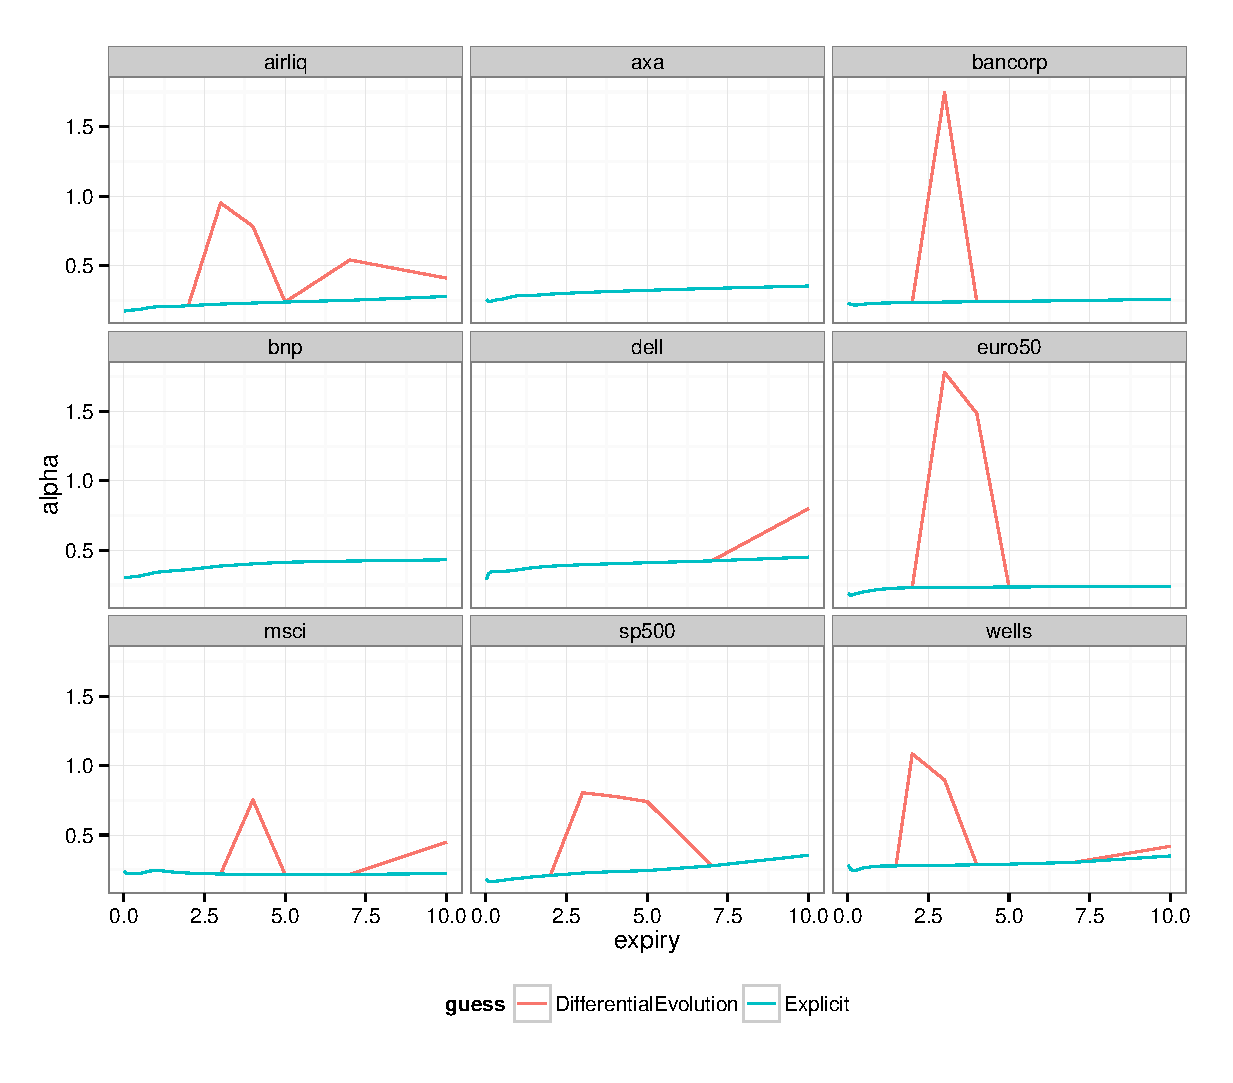
\includegraphics[width=12cm]{explicit_de_equity_alpha.eps}
\end{center}
\end{figure}


\subsubsection{Two SABRs for the same smile}
%the problem with differential evolution

The fact that two different SABR parameters sets can lead to smiles with nearly the same error measure is the root of issues with differential evolution: it is not obvious which set of parameter is the right one without some additional constraint on the variation of the parameters. This can be resolved by some penalty term, but it is difficult in practice to find the correct penalty term that works for a variety of situations. A better approach is to look beyond the best candidate, and consider as alternative initial guesses the other candidates in the latest generation with very similar error measure and different (lower) $\alpha$.

\subsubsection{Swaption smiles}
We apply the same calibration methodology as for the equity smiles cases, but relying on the normal formula with $\beta=\frac{1}{2}$ instead. The calibrated parameters are indistinguishable for between the calibration on the explicit initial guess and the calibration on the guess found by differential evolution (see Table XXX). Furthermore, the initial guess is very close to the calibration result. 

Figures \ref{fig:explicit_fit_1m_beta05} and \ref{fig:explicit_fit_2y_beta05} show how close are the smile produced by the initial guess and the smile resulting from the Levenberg-Marquardt minimization.

\begin{figure}[htbp]
  \caption{\label{fig:explicit_fit_1m_beta05}Initial guess and calibrated smile for a May 2014 1m5y Swaption }
\begin{center}
 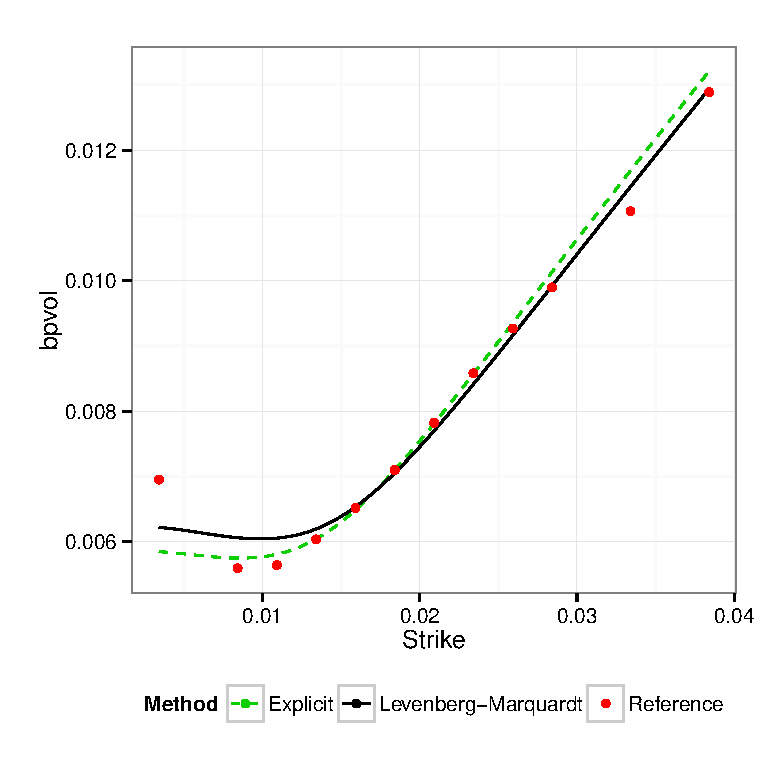
\includegraphics[width=8cm]{explicit_fit_1m_beta05.eps}
\end{center}
\end{figure}
\begin{figure}[htbp]
  \caption{\label{fig:explicit_fit_2y_beta05}Initial guess and calibrated smile for a May 2014 2y5y Swaption}
\begin{center}
 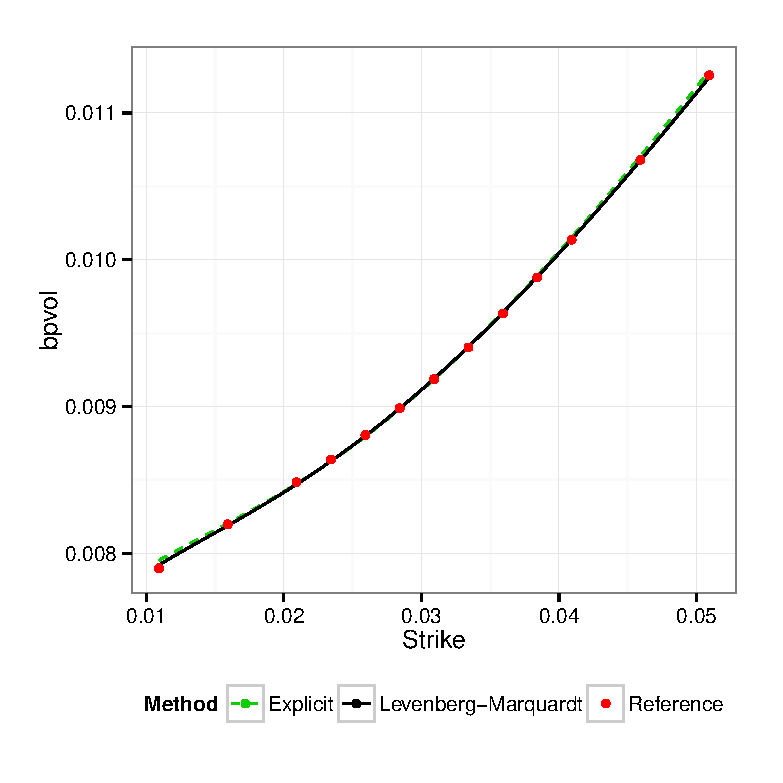
\includegraphics[width=8cm]{explicit_fit_2y_beta05.eps}
\end{center}
\end{figure}
\subsection{Calibration on the arbitrage free PDE}

\section{Conclusion}
\newpage
\bibliographystyle{rAMF}
%\bibliographystyle{ieeetr}
\bibliography{lefloch_smart_sabr}


\end{document}
